%%%%%%%%%%%%%%%%%%%%%%%%%%%%%%%%%%%%%%%%%
% a0poster Portrait Poster
% LaTeX Template
% Version 1.0 (22/06/13)
%
% The a0poster class was created by:
% Gerlinde Kettl and Matthias Weiser (tex@kettl.de)
% 
% This template has been downloaded from:
% http://www.LaTeXTemplates.com
%
% License:
% CC BY-NC-SA 3.0 (http://creativecommons.org/licenses/by-nc-sa/3.0/)
%
%%%%%%%%%%%%%%%%%%%%%%%%%%%%%%%%%%%%%%%%%
\documentclass[a0,portrait]{a0poster}
\usepackage{textcomp}
\usepackage{multirow}
\usepackage{tabularx}
\usepackage{multicol} % This is so we can have multiple columns of text side-by-side
\columnsep=100pt % This is the amount of white space between the columns in the poster
\columnseprule=3pt % This is the thickness of the black line between the columns in the poster

\usepackage[svgnames]{xcolor} 
\usepackage{times}
\usepackage{graphicx}
\graphicspath{{figures/}}
\usepackage{booktabs} 
\usepackage[font=small,labelfont=bf]{caption} % Required for specifying captions to tables and figures
\usepackage{amsfonts, amsmath, amsthm, amssymb} % For math fonts, symbols and environments
\usepackage{wrapfig} % Allows wrapping text around tables and figures
%\usepackage[theorems,skins]{tcolorbox}
\usepackage{empheq}
\usepackage{mdframed}
\fboxrule=10pt%border thickness
\usepackage{colortbl}
\usepackage[superscript,biblabel]{cite}

\begin{document}

%----------------------------------------------------------------------------------------
%	POSTER HEADER 
%----------------------------------------------------------------------------------------

% The header is divided into two boxes:
% The first is 75% wide and houses the title, subtitle, names, university/organization and contact information
% The second is 25% wide and houses a logo for your university/organization or a photo of you
% The widths of these boxes can be easily edited to accommodate your content as you see fit

\noindent
\begin{minipage}[b]{0.8\linewidth}
{\veryHuge\color{NavyBlue} \textbf{DELPHI: accurate deep ensemble model for protein interaction sites prediction}}\\ % Title

\smallskip

\noindent
\begin{minipage}[m]{0.5\linewidth}
 \color{Black}
\huge \textbf{Yiwei Li$^1$, G.~Brian Golding$^2$, and Lucian Ilie$^{1*}$}\\ % Author(s)
\huge $^1$ University of Western Ontario, CANADA\\ % University/organization
\huge $^2$ McMaster University, CANADA\\ % University/organization
%\Large \texttt{nkhiste@uwo.ca, ilie@uwo.ca}\\
{\normalsize $^*$Corresponding author: \texttt{ilie@uwo.ca}}
\end{minipage}
%
\begin{minipage}[m]{0.5\linewidth}
%\hspace{9cm}

\includegraphics[width=12cm]{uwo_logo.jpg}

\includegraphics[width=11cm]{Poster_Li/figures/mcmaster_logo.png}\\
\end{minipage}
\end{minipage}
\begin{minipage}[b]{0.2\linewidth}
\hfill
\includegraphics[width=10cm]{Poster_Li/figures/ismb2020.jpg}
\end{minipage}

\vspace{1cm} % A bit of extra whitespace between the header and poster content

%----------------------------------------------------------------------------------------

\begin{multicols}{2} % This is how many columns your poster will be broken into, a portrait poster is generally split into 2 columns

%----------------------------------------------------------------------------------------
%	ABSTRACT
%----------------------------------------------------------------------------------------

%\iffalse
%----------------------------------------------------------------------------------------
%	INTRODUCTION
%----------------------------------------------------------------------------------------

%\color{NavyBlue} % NavyBlue color for the introduction
\begin{mdframed}[linewidth=7pt]

\vspace*{-30pt}

\section*{\color{NavyBlue}Abstract}
\begin{itemize}
  \item Protein-protein interaction (PPI) binding sites prediction -- an vital problem in system biology
  \begin{itemize}
  \item Experimental methods are time and labor intensive
  \item Many computational approaches are proposed: sequence-based ones are very promising
  \item The prediction performance of current programs are far from satisfaction
  \end{itemize}
  \item {\color{NavyBlue}\textbf{DELPHI} - a new sequence-based Deep Learning model for PPI binding sites prediction} 
  \begin{itemize}
   \item A novel ensemble model architecture
   \item Three novel features
  \item More accurate than the leading sequence-based programs
  \end{itemize}
\end{itemize}
\end{mdframed}

\begin{mdframed}[linewidth=7pt]

\vspace*{-30pt}

\section*{\color{NavyBlue}Results}
\centering
%\begin{minipage}{0.6\linewidth}
\resizebox{0.65\textwidth}{!}{\begin{tabular}{@{}l*{5}{r}@{}}
    \toprule
    Dataset & Proteins & \multicolumn{3}{c}{Residues} & \multicolumn{1}{c@{}}{binding} \\ \cline{3-5}
    & & total & binding & non-binding & \multicolumn{1}{c@{}}{\% of total}\\ \hline
    Dset\_448\cite{zhang2019scriber} & 448   & 116,500 & 15,810 & 100,690 & 13.57 \\
    Dset\_355 & 355   & 95,940 & 11,467 & 84,473 & 11.95 \\
    Dset\_186\cite{murakami2010applying} & 186   & 36,219 & 5,517 & 30,702 & 15.23 \\
    Dset\_72\cite{murakami2010applying} & 72    & 18,140 & 1,923 & 16,217 & 10.60 \\
    Dset\_164\cite{dhole2014sequence} & 164   & 33,681 & 6,096 & 27,585 & 18.10 \\
    Train+Validate & 9,982 & 4,254,198 & 427,687 & 3,826,511 & 10.05 \\
    \hline
    \end{tabular}}
\captionof{table}{\color{Green} The datasets used for training, validation, and testing. The columns give, in order, the dataset names, the number of proteins in each dataset, the total number of residues, the number of binding, and the number of non-binding residues in each dataset, and the percentage of the binding residues out of total.\label{table:datasets}}
\end{mdframed}

\begin{mdframed}[linewidth=7pt]
\begin{minipage}[b]{0.48\linewidth}
\centering
\footnotesize
\captionof{table}{\color{Green} Performance comparison on Dset\_448 and Dset\_355. Programs are sorted in ascending order by AUPRC. Darker colours represent better results. The evaluation of the programs marked with ${}^*$ is by  Zhang\cite{zhang2019scriber}.  \label{tab:high_spec}}
    \resizebox{0.95\textwidth}{!}{\begin{tabular}{@{}l@{\ }*{8}{r}}
    \toprule
    \multicolumn{1}{@{}l}{Predictor} & \multicolumn{1}{c}{$\!$Sens.} & \multicolumn{1}{c}{Spec.} & \multicolumn{1}{c}{Prec.} & \multicolumn{1}{c}{Acc.} & \multicolumn{1}{c}{F1} & \multicolumn{1}{c}{MCC} & \multicolumn{1}{c}{$\!\!\!$AUROC$\!\!\!$} & \multicolumn{1}{c@{}}{$\!$AUPRC} \\
    \hline
    \multicolumn{9}{c}{Dset\_448} \\
    \hline
   SPPIDER\cite{porollo2007prediction}* & \cellcolor[rgb]{ .933,  .953,  .922}0.202 & 0.870 & \cellcolor[rgb]{ .961,  .973,  .957}0.194 & 0.781 & \cellcolor[rgb]{ .949,  .965,  .937}0.198 & \cellcolor[rgb]{ .957,  .969,  .949}0.071 & 0.517 & 0.159 \\
    SPRINT\cite{taherzadeh2016sequence}* & 0.183 & \cellcolor[rgb]{ .937,  .953,  .925}0.873 & 0.183 & 0.781 & 0.183 & 0.057 & \cellcolor[rgb]{ .839,  .882,  .812}0.570 & \cellcolor[rgb]{ .973,  .98,  .965}0.167 \\
    PSIVER\cite{murakami2010applying}* & \cellcolor[rgb]{ .973,  .98,  .969}0.191 & \cellcolor[rgb]{ .918,  .937,  .902}0.874 & \cellcolor[rgb]{ .973,  .98,  .969}0.191 & \cellcolor[rgb]{ .973,  .98,  .969}0.783 & \cellcolor[rgb]{ .973,  .98,  .969}0.191 & \cellcolor[rgb]{ .973,  .98,  .969}0.066 & \cellcolor[rgb]{ .808,  .859,  .773}0.581 & \cellcolor[rgb]{ .961,  .973,  .953}0.170 \\
    SPRINGS\cite{singh2014springs}* & \cellcolor[rgb]{ .839,  .882,  .808}0.229 & \cellcolor[rgb]{ .745,  .812,  .698}0.882 & \cellcolor[rgb]{ .843,  .886,  .812}0.228 & \cellcolor[rgb]{ .792,  .847,  .753}0.796 & \cellcolor[rgb]{ .839,  .882,  .808}0.229 & \cellcolor[rgb]{ .835,  .878,  .804}0.111 & \cellcolor[rgb]{ .675,  .761,  .612}0.625 & \cellcolor[rgb]{ .843,  .886,  .816}0.201 \\
    LORIS\cite{dhole2014sequence}* & \cellcolor[rgb]{ .714,  .792,  .659}0.264 & \cellcolor[rgb]{ .635,  .733,  .569}0.887 & \cellcolor[rgb]{ .718,  .792,  .663}0.263 & \cellcolor[rgb]{ .667,  .757,  .604}0.805 & \cellcolor[rgb]{ .718,  .792,  .663}0.263 & \cellcolor[rgb]{ .71,  .788,  .655}0.151 & \cellcolor[rgb]{ .58,  .694,  .502}0.656 & \cellcolor[rgb]{ .741,  .812,  .694}0.228 \\
    CRFPPI\cite{wei2015cascade}* & \cellcolor[rgb]{ .698,  .78,  .643}0.268 & \cellcolor[rgb]{ .635,  .733,  .569}0.887 & \cellcolor[rgb]{ .714,  .792,  .659}0.264 & \cellcolor[rgb]{ .667,  .757,  .604}0.805 & \cellcolor[rgb]{ .706,  .784,  .651}0.266 & \cellcolor[rgb]{ .698,  .78,  .643}0.154 & \cellcolor[rgb]{ .502,  .635,  .412}0.681 & \cellcolor[rgb]{ .706,  .784,  .651}0.238 \\
    SSWRF\cite{wei2016protein}* & \cellcolor[rgb]{ .627,  .729,  .561}0.288 & \cellcolor[rgb]{ .549,  .671,  .471}0.891 & \cellcolor[rgb]{ .635,  .733,  .569}0.286 & \cellcolor[rgb]{ .584,  .694,  .506}0.811 & \cellcolor[rgb]{ .631,  .729,  .565}0.287 & \cellcolor[rgb]{ .624,  .725,  .557}0.178 & \cellcolor[rgb]{ .482,  .624,  .388}0.687 & \cellcolor[rgb]{ .639,  .737,  .573}0.256 \\
    SCRIBER\cite{zhang2019scriber} & \cellcolor[rgb]{ .463,  .608,  .365}0.334 & \cellcolor[rgb]{ .443,  .592,  .341}0.896 & \cellcolor[rgb]{ .471,  .612,  .373}0.332 & \cellcolor[rgb]{ .443,  .592,  .341}0.821 & \cellcolor[rgb]{ .467,  .612,  .369}0.333 & \cellcolor[rgb]{ .463,  .608,  .365}0.230 & \cellcolor[rgb]{ .4,  .561,  .29}0.715 & \cellcolor[rgb]{ .522,  .651,  .435}0.287 \\
    DELPHI & \cellcolor[rgb]{ .329,  .51,  .208}0.371 & \cellcolor[rgb]{ .329,  .51,  .208}0.901 & \cellcolor[rgb]{ .329,  .51,  .208}0.371 & \cellcolor[rgb]{ .329,  .51,  .208}0.829 & \cellcolor[rgb]{ .329,  .51,  .208}0.371 & \cellcolor[rgb]{ .329,  .51,  .208}0.272 & \cellcolor[rgb]{ .329,  .51,  .208}0.737 & \cellcolor[rgb]{ .329,  .51,  .208}0.337 \\
    \hline
    \multicolumn{9}{c}{Dset\_355} \\
    \hline
    SPPIDER & \cellcolor[rgb]{ .961,  .973,  .957}0.180 & \cellcolor[rgb]{ .949,  .965,  .941}0.889 & \cellcolor[rgb]{ .961,  .973,  .953}0.180 & \cellcolor[rgb]{ .957,  .969,  .949}0.804 & \cellcolor[rgb]{ .961,  .973,  .953}0.180 & \cellcolor[rgb]{ .961,  .973,  .953}0.068 & 0.515 & 0.138 \\
    SPRINT & 0.168 & 0.886 & 0.167 & 0.801 & 0.168 & 0.054 & \cellcolor[rgb]{ .839,  .882,  .808}0.571 & \cellcolor[rgb]{ .961,  .973,  .953}0.150 \\
    PSIVER & \cellcolor[rgb]{ .969,  .976,  .965}0.178 & \cellcolor[rgb]{ .965,  .976,  .957}0.888 & \cellcolor[rgb]{ .969,  .976,  .965}0.177 & \cellcolor[rgb]{ .969,  .976,  .961}0.803 & \cellcolor[rgb]{ .969,  .976,  .965}0.177 & \cellcolor[rgb]{ .969,  .976,  .965}0.065 & \cellcolor[rgb]{ .804,  .859,  .769}0.583 & \cellcolor[rgb]{ .941,  .957,  .929}0.155 \\
    SPRINGS & \cellcolor[rgb]{ .855,  .894,  .827}0.211 & \cellcolor[rgb]{ .867,  .906,  .843}0.892 & \cellcolor[rgb]{ .859,  .898,  .831}0.210 & \cellcolor[rgb]{ .863,  .898,  .835}0.811 & \cellcolor[rgb]{ .855,  .894,  .827}0.211 & \cellcolor[rgb]{ .855,  .894,  .831}0.103 & \cellcolor[rgb]{ .733,  .804,  .682}0.608 & \cellcolor[rgb]{ .859,  .898,  .831}0.178 \\
    LORIS & \cellcolor[rgb]{ .749,  .816,  .706}0.242 & \cellcolor[rgb]{ .769,  .831,  .725}0.896 & \cellcolor[rgb]{ .757,  .82,  .71}0.240 & \cellcolor[rgb]{ .761,  .824,  .714}0.818 & \cellcolor[rgb]{ .753,  .82,  .706}0.241 & \cellcolor[rgb]{ .753,  .82,  .71}0.137 & \cellcolor[rgb]{ .647,  .745,  .584}0.637 & \cellcolor[rgb]{ .773,  .835,  .729}0.203 \\
    CRFPPI & \cellcolor[rgb]{ .733,  .804,  .686}0.247 & \cellcolor[rgb]{ .741,  .812,  .698}0.897 & \cellcolor[rgb]{ .737,  .808,  .69}0.245 & \cellcolor[rgb]{ .737,  .808,  .69}0.819 & \cellcolor[rgb]{ .733,  .808,  .686}0.246 & \cellcolor[rgb]{ .737,  .808,  .686}0.143 & \cellcolor[rgb]{ .573,  .69,  .498}0.662 & \cellcolor[rgb]{ .733,  .804,  .682}0.214 \\
    SSWRF & \cellcolor[rgb]{ .663,  .753,  .6}0.268 & \cellcolor[rgb]{ .655,  .749,  .592}0.901 & \cellcolor[rgb]{ .659,  .753,  .596}0.268 & \cellcolor[rgb]{ .659,  .749,  .596}0.825 & \cellcolor[rgb]{ .659,  .753,  .6}0.268 & \cellcolor[rgb]{ .659,  .753,  .596}0.168 & \cellcolor[rgb]{ .561,  .678,  .482}0.667 & \cellcolor[rgb]{ .682,  .769,  .624}0.228 \\
    DLPred\cite{zhang2019sequence} & \cellcolor[rgb]{ .522,  .651,  .435}0.308 & \cellcolor[rgb]{ .518,  .647,  .431}0.906 & \cellcolor[rgb]{ .522,  .651,  .435}0.308 & \cellcolor[rgb]{ .514,  .647,  .427}0.835 & \cellcolor[rgb]{ .522,  .651,  .435}0.308 & \cellcolor[rgb]{ .522,  .651,  .435}0.214 & \cellcolor[rgb]{ .396,  .561,  .286}0.724 & \cellcolor[rgb]{ .525,  .655,  .439}0.272 \\
    SCRIBER & \cellcolor[rgb]{ .475,  .616,  .38}0.322 & \cellcolor[rgb]{ .475,  .616,  .38}0.908 & \cellcolor[rgb]{ .475,  .616,  .38}0.322 & \cellcolor[rgb]{ .475,  .616,  .376}0.838 & \cellcolor[rgb]{ .475,  .616,  .38}0.322 & \cellcolor[rgb]{ .475,  .616,  .38}0.230 & \cellcolor[rgb]{ .408,  .569,  .302}0.719 & \cellcolor[rgb]{ .514,  .643,  .424}0.275 \\
    DELPHI & \cellcolor[rgb]{ .329,  .51,  .208}0.364 & \cellcolor[rgb]{ .329,  .51,  .208}0.914 & \cellcolor[rgb]{ .329,  .51,  .208}0.364 & \cellcolor[rgb]{ .329,  .51,  .208}0.848 & \cellcolor[rgb]{ .329,  .51,  .208}0.364 & \cellcolor[rgb]{ .329,  .51,  .208}0.278 & \cellcolor[rgb]{ .329,  .51,  .208}0.746 & \cellcolor[rgb]{ .329,  .51,  .208}0.326 \\
    \end{tabular}} \label{tab_comp_448_355}%
  \end{minipage}
\hfill
\begin{minipage}[b]{0.48\linewidth}
  \centering
\footnotesize
\captionof{table}{\color{Green}  Performance comparison on Dset\_186, Dset\_164, and Dset\_72 using the same metrics. Darker colours represent better results.}
    \resizebox{0.95\textwidth}{!}{\begin{tabular}{@{}l@{\ }*{8}{r}}
    \toprule
    \multicolumn{1}{@{}l}{Predictor} & \multicolumn{1}{c}{$\!$Sens.} & \multicolumn{1}{c}{Spec.} & \multicolumn{1}{c}{Prec.} & \multicolumn{1}{c}{Acc.} & \multicolumn{1}{c}{F1} & \multicolumn{1}{c}{MCC} & \multicolumn{1}{c}{$\!\!\!$AUROC$\!\!\!$} & \multicolumn{1}{c@{}}{$\!$AUPRC} \\
    \hline
    \multicolumn{9}{c}{Dset\_186} \\
    \hline
    SPPIDER & \cellcolor[rgb]{ .988,  .988,  1}0.194 & \cellcolor[rgb]{ .988,  .988,  1}0.848 & \cellcolor[rgb]{ .988,  .988,  1}0.186 & \cellcolor[rgb]{ .988,  .988,  1}0.748 & \cellcolor[rgb]{ .988,  .988,  1}0.190 & \cellcolor[rgb]{ .988,  .988,  1}0.041 & \cellcolor[rgb]{ .988,  .988,  1}0.499 & \cellcolor[rgb]{ .988,  .988,  1}0.165 \\
    SCRIBER & \cellcolor[rgb]{ .631,  .729,  .573}0.279 & \cellcolor[rgb]{ .576,  .69,  .506}0.870 & \cellcolor[rgb]{ .62,  .722,  .557}0.279 & \cellcolor[rgb]{ .604,  .71,  .537}0.780 & \cellcolor[rgb]{ .624,  .725,  .565}0.279 & \cellcolor[rgb]{ .62,  .722,  .557}0.150 & \cellcolor[rgb]{ .529,  .655,  .447}0.647 & \cellcolor[rgb]{ .643,  .741,  .588}0.246 \\
    DLPred & \cellcolor[rgb]{ .459,  .604,  .365}0.320 & \cellcolor[rgb]{ .439,  .592,  .341}0.878 & \cellcolor[rgb]{ .455,  .6,  .357}0.320 & \cellcolor[rgb]{ .451,  .6,  .357}0.793 & \cellcolor[rgb]{ .459,  .604,  .361}0.320 & \cellcolor[rgb]{ .455,  .604,  .361}0.198 & \cellcolor[rgb]{ .38,  .549,  .267}0.694 & \cellcolor[rgb]{ .459,  .604,  .361}0.290 \\
    DELPHI & \cellcolor[rgb]{ .329,  .51,  .208}0.351 & \cellcolor[rgb]{ .329,  .51,  .208}0.884 & \cellcolor[rgb]{ .329,  .51,  .208}0.351 & \cellcolor[rgb]{ .329,  .51,  .208}0.803 & \cellcolor[rgb]{ .329,  .51,  .208}0.351 & \cellcolor[rgb]{ .329,  .51,  .208}0.235 & \cellcolor[rgb]{ .329,  .51,  .208}0.710 & \cellcolor[rgb]{ .329,  .51,  .208}0.319 \\
    \hline
    \multicolumn{9}{c}{Dset\_164} \\
    \hline
    SPPIDER & \cellcolor[rgb]{ .761,  .824,  .729}0.264 & \cellcolor[rgb]{ .949,  .961,  .953}0.828 & \cellcolor[rgb]{ .812,  .859,  .788}0.253 & \cellcolor[rgb]{ .859,  .894,  .843}0.726 & \cellcolor[rgb]{ .788,  .843,  .757}0.258 & \cellcolor[rgb]{ .804,  .855,  .776}0.090 & \cellcolor[rgb]{ .988,  .988,  1}0.528 & \cellcolor[rgb]{ .914,  .933,  .91}0.220 \\
    PSIVER & \cellcolor[rgb]{ .988,  .988,  1}0.217 & \cellcolor[rgb]{ .988,  .988,  1}0.826 & \cellcolor[rgb]{ .988,  .988,  1}0.216 & \cellcolor[rgb]{ .988,  .988,  1}0.716 & \cellcolor[rgb]{ .988,  .988,  1}0.216 & \cellcolor[rgb]{ .988,  .988,  1}0.043 & \cellcolor[rgb]{ .878,  .91,  .867}0.554 & \cellcolor[rgb]{ .988,  .988,  1}0.205 \\
    SSWRF & \cellcolor[rgb]{ .753,  .816,  .714}0.266 & \cellcolor[rgb]{ .741,  .808,  .702}0.838 & \cellcolor[rgb]{ .749,  .816,  .714}0.266 & \cellcolor[rgb]{ .745,  .812,  .71}0.734 & \cellcolor[rgb]{ .749,  .816,  .714}0.266 & \cellcolor[rgb]{ .749,  .816,  .714}0.103 & \cellcolor[rgb]{ .663,  .753,  .608}0.606 & \cellcolor[rgb]{ .796,  .847,  .769}0.243 \\
    CRFPPI & \cellcolor[rgb]{ .682,  .769,  .631}0.280 & \cellcolor[rgb]{ .675,  .761,  .62}0.841 & \cellcolor[rgb]{ .682,  .765,  .631}0.280 & \cellcolor[rgb]{ .678,  .765,  .627}0.739 & \cellcolor[rgb]{ .682,  .765,  .631}0.280 & \cellcolor[rgb]{ .682,  .765,  .631}0.121 & \cellcolor[rgb]{ .655,  .745,  .596}0.608 & \cellcolor[rgb]{ .667,  .757,  .612}0.267 \\
    SCRIBER & \cellcolor[rgb]{ .451,  .6,  .353}0.327 & \cellcolor[rgb]{ .451,  .596,  .353}0.851 & \cellcolor[rgb]{ .451,  .6,  .353}0.327 & \cellcolor[rgb]{ .451,  .6,  .353}0.756 & \cellcolor[rgb]{ .451,  .6,  .353}0.327 & \cellcolor[rgb]{ .451,  .6,  .353}0.179 & \cellcolor[rgb]{ .451,  .596,  .353}0.657 & \cellcolor[rgb]{ .49,  .627,  .4}0.301 \\
    DLPred & \cellcolor[rgb]{ .4,  .561,  .294}0.338 & \cellcolor[rgb]{ .4,  .561,  .29}0.854 & \cellcolor[rgb]{ .4,  .561,  .29}0.338 & \cellcolor[rgb]{ .4,  .561,  .29}0.760 & \cellcolor[rgb]{ .4,  .561,  .294}0.338 & \cellcolor[rgb]{ .4,  .561,  .29}0.192 & \cellcolor[rgb]{ .384,  .549,  .275}0.672 & \cellcolor[rgb]{ .341,  .518,  .22}0.330 \\
    DELPHI & \cellcolor[rgb]{ .329,  .51,  .208}0.352 & \cellcolor[rgb]{ .329,  .51,  .208}0.857 & \cellcolor[rgb]{ .329,  .51,  .208}0.352 & \cellcolor[rgb]{ .329,  .51,  .208}0.765 & \cellcolor[rgb]{ .329,  .51,  .208}0.352 & \cellcolor[rgb]{ .329,  .51,  .208}0.209 & \cellcolor[rgb]{ .329,  .51,  .208}0.685 & \cellcolor[rgb]{ .329,  .51,  .208}0.332 \\
    \hline
    \multicolumn{9}{c}{Dset\_72} \\
    \hline
    SPPIDER & \cellcolor[rgb]{ .8,  .851,  .773}0.188 & \cellcolor[rgb]{ .988,  .988,  1}0.898 & \cellcolor[rgb]{ .843,  .882,  .827}0.179 & \cellcolor[rgb]{ .925,  .945,  .925}0.823 & \cellcolor[rgb]{ .824,  .867,  .8}0.183 & \cellcolor[rgb]{ .835,  .878,  .816}0.084 & \cellcolor[rgb]{ .988,  .988,  1}0.522 & \cellcolor[rgb]{ .988,  .988,  1}0.134 \\
    PSIVER & \cellcolor[rgb]{ .988,  .988,  1}0.152 & \cellcolor[rgb]{ .937,  .953,  .937}0.899 & \cellcolor[rgb]{ .988,  .988,  1}0.152 & \cellcolor[rgb]{ .988,  .988,  1}0.820 & \cellcolor[rgb]{ .988,  .988,  1}0.152 & \cellcolor[rgb]{ .988,  .988,  1}0.052 & \cellcolor[rgb]{ .706,  .784,  .659}0.604 & \cellcolor[rgb]{ .941,  .957,  .945}0.141 \\
    CRFPPI & \cellcolor[rgb]{ .475,  .616,  .384}0.248 & \cellcolor[rgb]{ .478,  .62,  .388}0.911 & \cellcolor[rgb]{ .475,  .616,  .384}0.248 & \cellcolor[rgb]{ .49,  .627,  .4}0.840 & \cellcolor[rgb]{ .475,  .616,  .384}0.248 & \cellcolor[rgb]{ .478,  .616,  .384}0.158 & \cellcolor[rgb]{ .475,  .616,  .384}0.669 & \cellcolor[rgb]{ .565,  .682,  .49}0.200 \\
    SSWRF & \cellcolor[rgb]{ .482,  .624,  .392}0.246 & \cellcolor[rgb]{ .486,  .624,  .396}0.911 & \cellcolor[rgb]{ .482,  .624,  .392}0.246 & \cellcolor[rgb]{ .498,  .635,  .412}0.840 & \cellcolor[rgb]{ .482,  .624,  .392}0.246 & \cellcolor[rgb]{ .486,  .624,  .396}0.157 & \cellcolor[rgb]{ .447,  .596,  .349}0.678 & \cellcolor[rgb]{ .576,  .69,  .506}0.198 \\
    SCRIBER & \cellcolor[rgb]{ .557,  .675,  .482}0.232 & \cellcolor[rgb]{ .553,  .671,  .475}0.909 & \cellcolor[rgb]{ .557,  .675,  .482}0.232 & \cellcolor[rgb]{ .569,  .686,  .498}0.837 & \cellcolor[rgb]{ .557,  .675,  .482}0.232 & \cellcolor[rgb]{ .557,  .678,  .482}0.141 & \cellcolor[rgb]{ .439,  .592,  .341}0.680 & \cellcolor[rgb]{ .576,  .69,  .506}0.198 \\
    DLPred & \cellcolor[rgb]{ .482,  .62,  .392}0.246 & \cellcolor[rgb]{ .859,  .894,  .843}0.901 & \cellcolor[rgb]{ .482,  .62,  .388}0.246 & \cellcolor[rgb]{ .855,  .894,  .839}0.826 & \cellcolor[rgb]{ .482,  .62,  .388}0.246 & \cellcolor[rgb]{ .529,  .655,  .447}0.148 & \cellcolor[rgb]{ .412,  .569,  .306}0.688 & \cellcolor[rgb]{ .467,  .612,  .373}0.215 \\
    DELPHI & \cellcolor[rgb]{ .329,  .51,  .208}0.274 & \cellcolor[rgb]{ .329,  .51,  .208}0.914 & \cellcolor[rgb]{ .329,  .51,  .208}0.274 & \cellcolor[rgb]{ .329,  .51,  .208}0.847 & \cellcolor[rgb]{ .329,  .51,  .208}0.274 & \cellcolor[rgb]{ .329,  .51,  .208}0.189 & \cellcolor[rgb]{ .329,  .51,  .208}0.711 & \cellcolor[rgb]{ .329,  .51,  .208}0.237 \\
\label{tab_ds186_164_72}
    \end{tabular}}
    \end{minipage}
\end{mdframed}

\begin{mdframed}[linewidth=7pt]
\begin{minipage}[b]{0.48\linewidth}
%\raggedright
%\vspace*{10pt}
\centering 
\hspace*{40pt}{\includegraphics[width=0.8\linewidth]{Poster_Li/remove_features_individually_Testing.pdf}}
\vspace*{10pt}
\captionof{figure}{\color{Green}The areas under PR curves with the removal of one out of the twelve features on Dset\_448. One feature is removed each time, and the DELPHI model is trained, validated, and tested using the remaining eleven features. The x-axis shows the removed features where 'None' indicates using all twelve features, and the y-axis is the AUPRC achieved. The features are sorted decreasingly by the AUPRC values. \label{fig:remove_feature}}
\end{minipage}
\hfill
\begin{minipage}[b]{0.48\linewidth}
%\raggedleft
%\vspace*{-30pt}
\centering 
\color{Black}{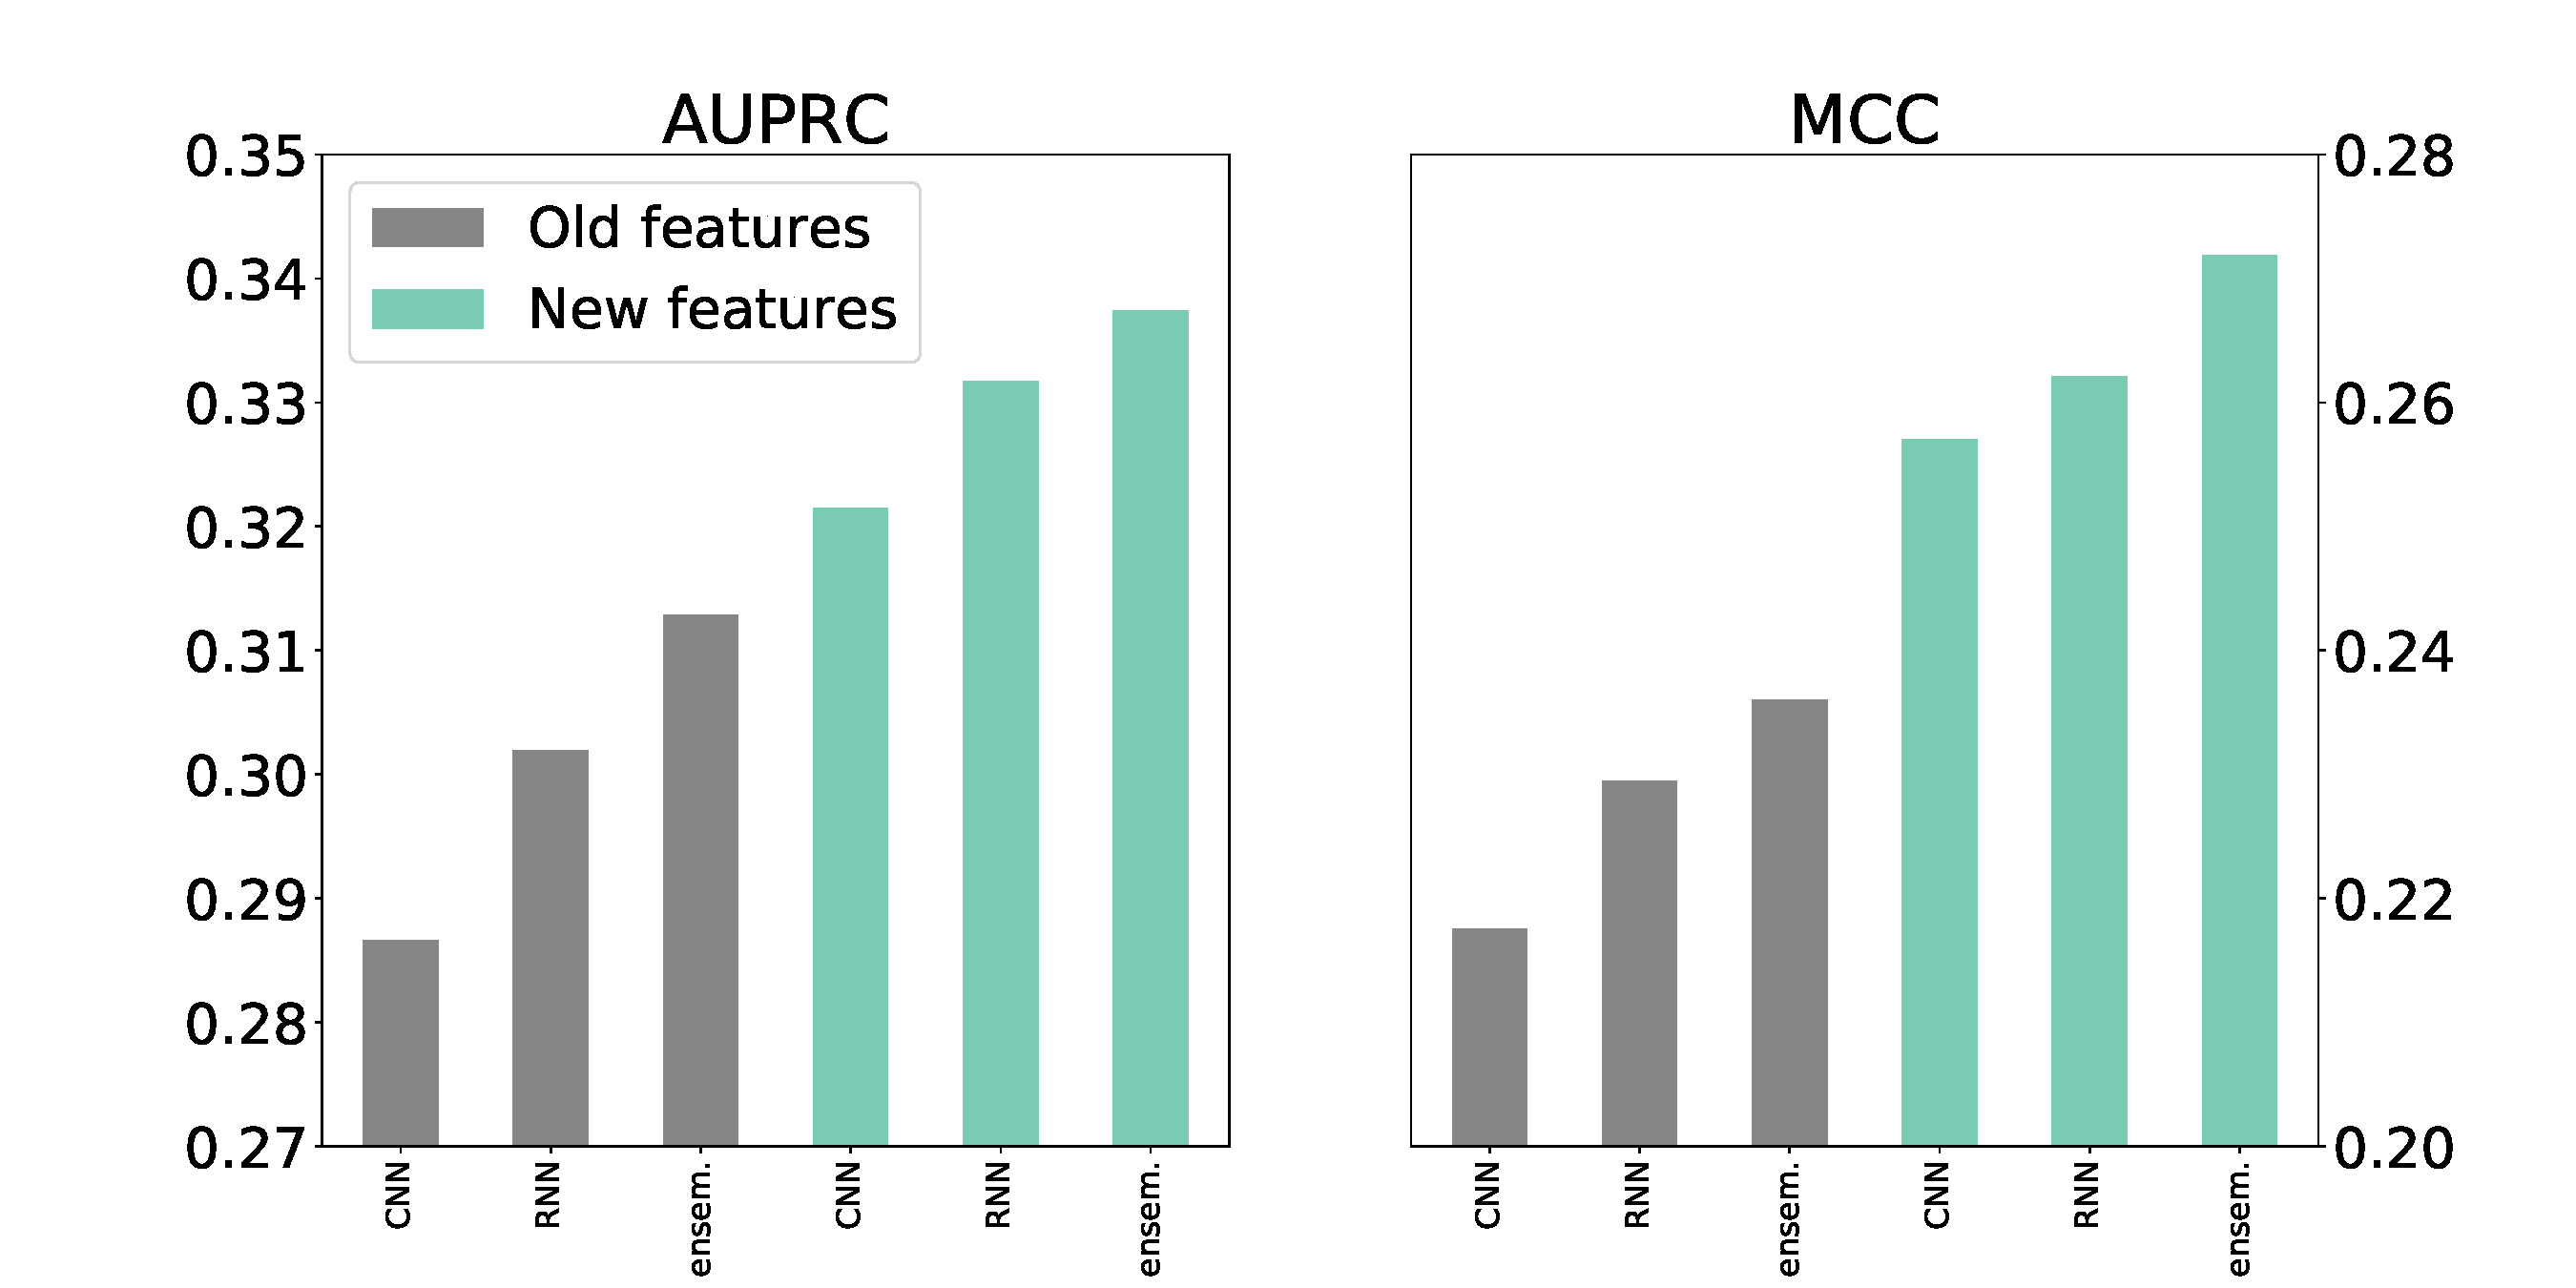
\includegraphics[width=0.95\linewidth]{Poster_Li/CNN_RNN_ensemble.pdf}}
\captionof{figure}{\color{Green} The evaluation of the DELPHI model architecture and the three novel features. The area under PR curves (left) and MCC (right) are plotted separately. Each plot contains the performance of using CNN, RNN, and the ensemble model on Dset\_448. Two different colors indicate with and without the three new features.\label{fig:cnn_rnn_feature_evaluation}}
\end{minipage}
\end{mdframed}

\begin{mdframed}[linewidth=7pt]
\begin{center}
\color{Black}{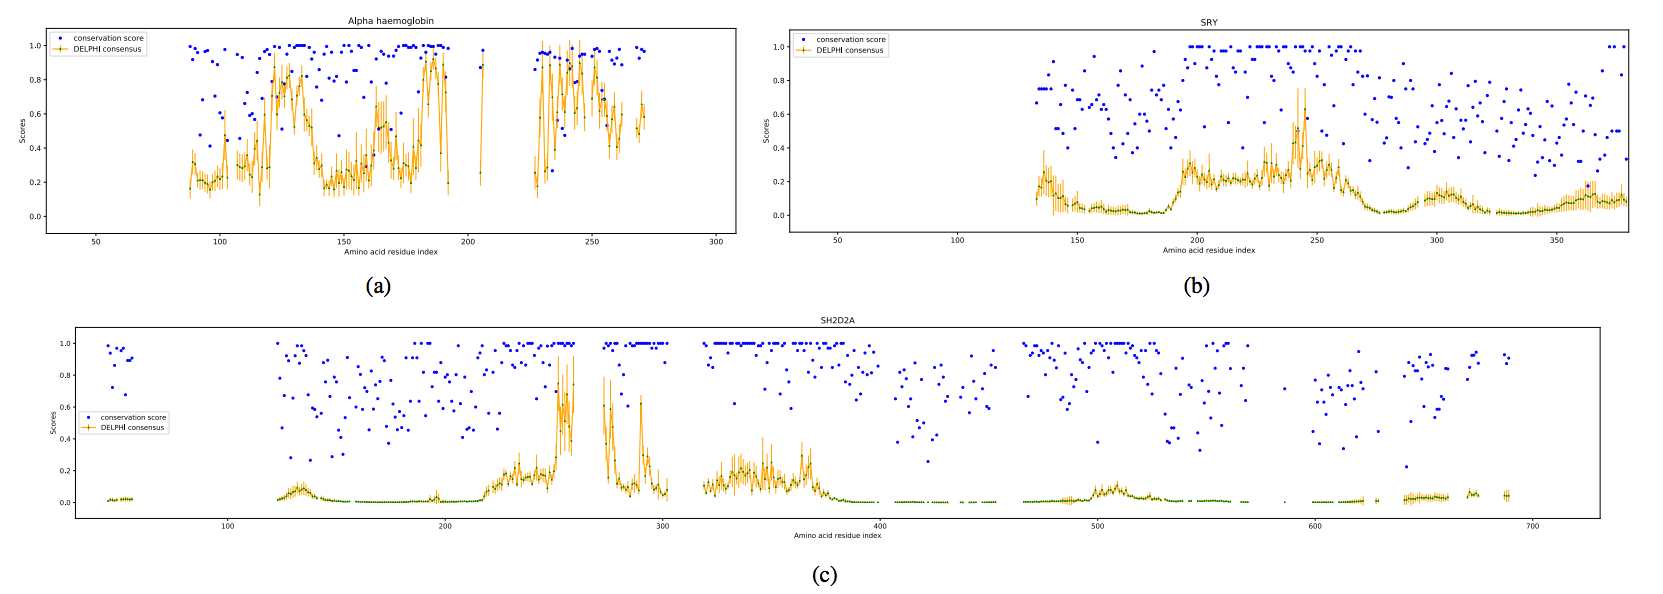
\includegraphics[width=1.0\linewidth]{Poster_Li/figures/combined_conver.png}}
\captionof{figure}{\color{Green} Three proteins were evaluated to compare the PPI
predicted by DELPHI (green and orange) with the degree of site-by-site conservation
(blue).  Only sites represented in ten or more taxa are included resulting
in some apparent gaps.  The proteins are (a) alpha haemoglobin, (b) SRY
and (c) SH2D2A. \label{fig:conservation}}
\end{center}
\end{mdframed}

%----------------------------------------------------------------------------------------
%	MATERIALS AND METHODS
%----------------------------------------------------------------------------------------

\begin{mdframed}[linewidth=7pt]
%\color{NavyBlue}

\vspace*{-30pt}

\section*{\color{NavyBlue} Methods}
\subsection*{Model Architecture} 
\begin{center}
\color{Black}{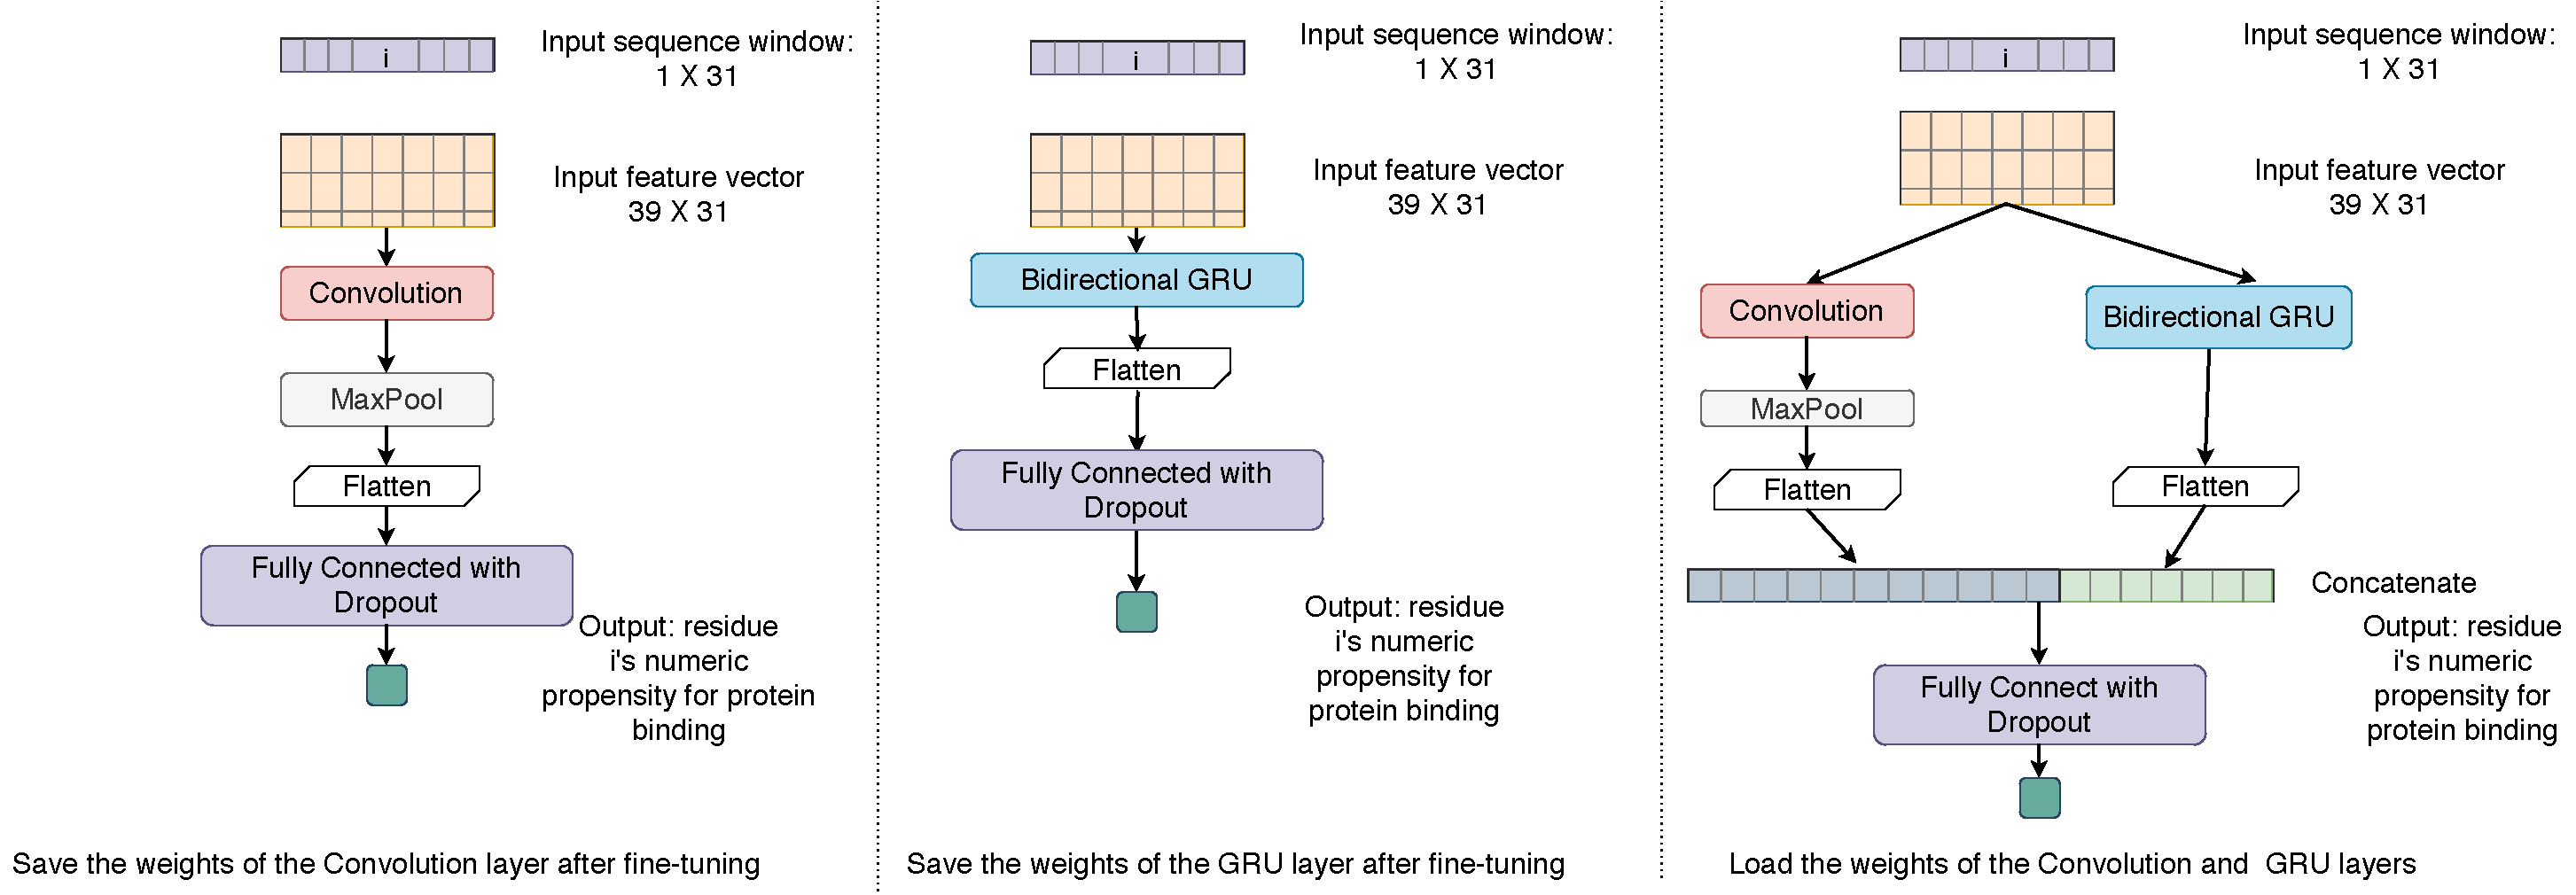
\includegraphics[width=1.0\linewidth]{Poster_Li/Model_architecture.pdf}}
\captionof{figure}{\color{Green} The architecture of DELPHI. Left: the CNN component of the model. Middle: the RNN component of the model. Right: The ensemble model. \label{fig:model_arch}}
\end{center}
% \end{mdframed}
\subsection*{Model Input and Output} 
\begin{center}
\color{Black}{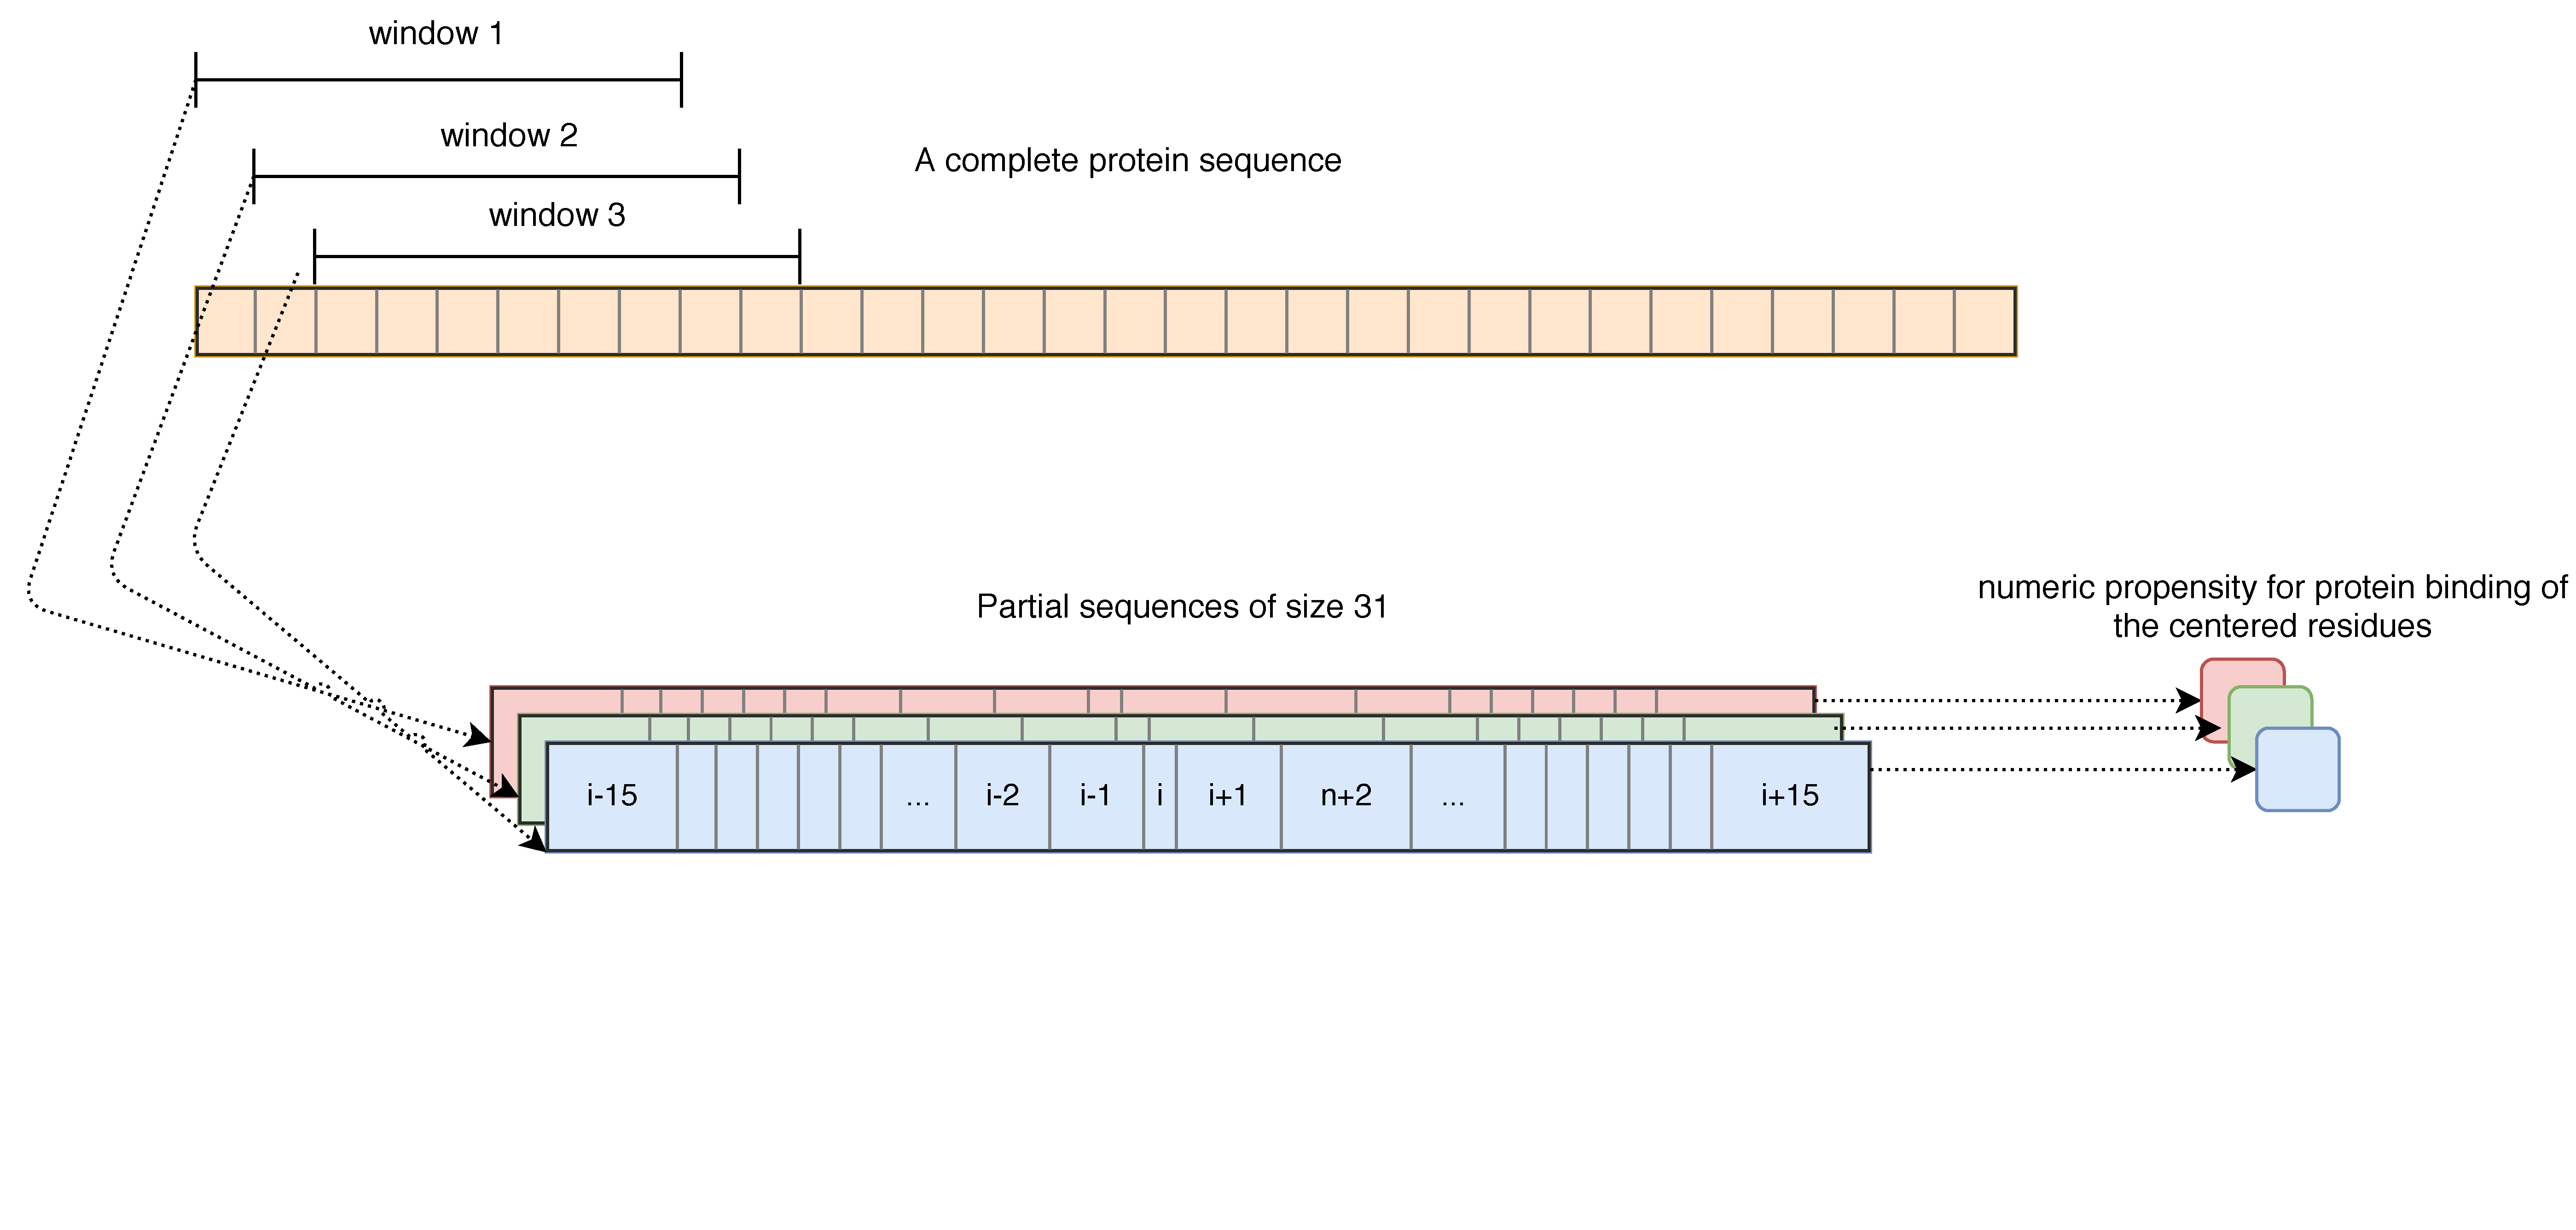
\includegraphics[width=1.0\linewidth]{Poster_Li/many_2_one.pdf}}
\captionof{figure}{\color{Green} The many-to-one prediction. Sliding windows of size 31, stride 1 are put on top of an input protein sequence. Each time, a sub-sequence of length 31 is extracted. The model predicts the protein-binding propensity of the middle amino acid for each sub-sequence. \label{fig:many_2_one}}
\end{center}

\subsection*{Input Features and the DELPHI Web Server} 
\begin{minipage}[b]{0.47\linewidth}
\begin{center}
    \resizebox{0.9\textwidth}{!}{\begin{tabular}{@{}ll@{}r@{}}
    \toprule
    Feature & Program & Dimension \\
    \midrule
    High-scoring segment pair (HSP) & Compute & 1 \\
    3-mer amino acid embedding (ProtVec1D) & Load/compute & 1 \\
    Position information & Compute & 1 \\
    Position-specific scoring matrix (PSSM) & Psi-Blast & 20 \\
    Evolutionary conservation (ECO) & Hhblits & 1 \\
    Putative relative solvent accessibility (RSA) & ASAquick & 1 \\
    Relative amino acid propensity (RAA) & Load  & 1 \\
    Putative protein-binding disorder & ANCHOR & 1 \\
    Hydropathy index & Load  & 1 \\
    Physicochemical characteristics & Load  & 3 \\
    Physical properties & Load  & 7 \\
    PKx   & Load  & 1 \\
    \bottomrule
    \end{tabular}}
      \captionof{table}{\color{Green}The feature names, computation programs, and dimensions of each feature used by DELPHI. The first three features are novel.}
\end{center}
\end{minipage}
% \vspace*{-20pt}
\begin{minipage}[b]{0.48\linewidth}
\centering 
\color{Black}{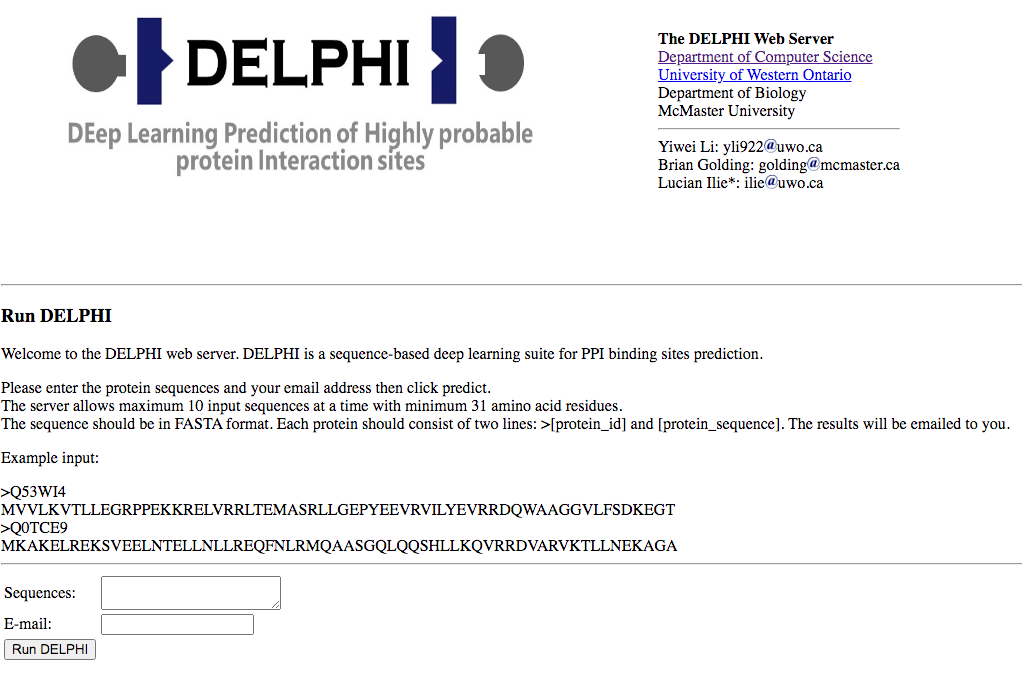
\includegraphics[width=\linewidth]{Poster_Li/figures/delphi_web.png}}
\captionof{figure}{\color{Green} The interface of the DELPHI web server. It takes protein sequences in FASTA format as input, and the result will be emailed to the user. \label{fig:web_server}}
\end{minipage}
\end{mdframed}

\begin{mdframed}[linewidth=7pt]
%----------------------------------------------------------------------------------------
%	CONCLUSIONS
%----------------------------------------------------------------------------------------
%\color{NavyBlue} % NavyBlue color for the conclusions to make them stand out

\vspace*{-30pt}
\section*{\color{NavyBlue}Conclusions}
\begin{itemize}
  \item DELPHI is a more accurate sequence-based PPI sites predictor.
  \item The three novel features and the ensemble architecture can be potentially used in other protein sequence classifiers. 
\end{itemize}
\end{mdframed}
\begin{mdframed}[linewidth=7pt]
\color{DarkSlateGray} % Set the color back to DarkSlateGray for the rest of the content
\footnotesize{
%----------------------------------------------------------------------------------------
%	FORTHCOMING RESEARCH
%----------------------------------------------------------------------------------------

\vspace*{-20pt}
\section*{Availability} 
The source code of DELPHI is freely available from \texttt{https://github.com/lucian-ilie/DELPHI/}.\\
All datasets and results as well the DELPHI web server is available from \texttt{www.csd.uwo.ca/\texttildelow{}yli922/index.php}.
\vspace*{-20pt}
\nocite{*} % Print all references regardless of whether they were cited in the poster or not
\bibliographystyle{plain} % Plain referencing style
\bibliography{poster} % Use the example bibliography file sample.bib
\vspace*{-30pt}
\section*{Acknowledgements}
The research of L.I. is funded by an NSERC Discovery Grant (R3143A01) and a Research Tools and Instruments Grant (R3143A07). The research of G.B.G. is funded by an NSERC Discovery Grant RGPIN-2020-05733.
}
%----------------------------------------------------------------------------------------
\end{mdframed}
\end{multicols}
\end{document}
